\documentclass[10pt]{beamer}

\usepackage[utf8]{inputenc}

\usepackage[T1]{fontenc}

\usepackage{microtype} % microtypographical enhancements

\usepackage[english]{babel}

\usepackage{amsmath, amssymb, amsthm, amsfonts}

\usepackage{graphicx}

\usepackage{bm} % boldface symbols (\bm)

\usepackage{twoopt} % for convenient commands

\usepackage{xfrac} % for \sfrac command

\usepackage{mathrsfs} % calligraphic font \mathscr{C}


\usepackage{dcolumn} % improved alignment of table columns

\usepackage{booktabs} % improved horizontal lines in tables

\usepackage[justification=centering]{caption} % center multiline captions or e.g. [format=hang]



\usepackage[style=alphabetic, backend=biber, isbn=false, url=false, doi=false]{biblatex}

\addbibresource{thesis.bib}


\usepackage{tikz}

\usetikzlibrary{positioning,decorations.markings}
\tikzset{croot/.style={circle,draw,fill=black,inner sep=0pt,minimum size=2mm},
	 nroot/.style={circle,draw,inner sep=0pt,minimum size=2mm},
	 node distance = 1
	 }



\input{pres_definitions}


\usepackage{threeparttable,array}

\newcolumntype{C}{>{$\displaystyle}c <{$}}


\usetheme[progressbar=frametitle]{metropolis}

\usepackage{appendixnumberbeamer}


\usepackage{booktabs}

\usepackage[scale=2]{ccicons}


\usepackage{pgfplots}

\usepgfplotslibrary{dateplot}


\usepackage{xspace}

\newcommand{\themename}{\textbf{\textsc{metropolis}}\xspace}


\title{Invariant differential operators \\ for 1-graded geometries}

%\subtitle{}

% \date{\today}

\date{}

\author{Vít Tuček}

\institute{Mathematical Institute of Charles University}

\titlegraphic{\hfill\includegraphics[height=2cm]{logo-en.pdf}}


\begin{document}

\metroset{titleformat frame=smallcaps}

\maketitle


\begin{frame}{Table of contents}

\setbeamertemplate{section in toc}[sections numbered]

\tableofcontents[hideallsubsections]

\end{frame}


%\begin{frame}{Animation}

% \begin{itemize}[<+- | alert@+>]

% \item \alert<4>{This is\only<4>{ really} important}

% \item Now this

% \item And now this

% \end{itemize}

%\end{frame}


\section{Hermitian symmetric spaces}


\begin{frame}{Definition -- Hermitian symmetric space}

\begin{itemize}[<+- | alert@+>]
\item Compact symmetric space $H/K$ is called a Hermitian symmetric space if it admits $H$-invariant complex structure
\item $H/K \simeq G/P$ where $G$ is a complexification of $H$ and $P$ is a parabolic subgroup with abelian radical
\item The noncompact dual $H^*$ is given on the level of Lie algebras by $\lie{h}^* = \lie{k} \oplus \imath \lie{m}$ where $\lie{h} = \lie{k} \oplus \lie{m}$
\item Borel embedding $H^*/K \hookrightarrow G/P$
\item Harish-Chandra embedding $H^*/K \hookrightarrow \lie{m}_+$ where $\lie{m}_+$ is the nilradical of $\lie{p}$
\end{itemize}

\end{frame}


\begin{frame}{Examples}

$
 I_{m,n} = \begin{pmatrix} \Id_m & 0 \\ 0 & -\Id_n \end{pmatrix} \quad J = \begin{pmatrix} 0 & \Id_n \\ -\Id_n & 0 \end{pmatrix} \quad X^\dag = \overline{X}^t
$
\pause

%\vspace{0.2cm}
\begin{equation*}
\begin{aligned}
\alert{\mathrm{SU}(p,q)} &= \{ g \in \mathrm{GL}(p +q, \mathbb{C}) \,|\, g I_{p,q}g^\dag = I_{p,q} \}\\[0.5cm]
\pause
\mathrm{Sp}(n, \mathbb{C}) &= \{ g \in \mathrm{GL}(2n, \mathbb{C}) \,|\, g^t J g  = J \}\\
\alert{\mathrm{Sp}(n, \mathbb{R})} &= \mathrm{Sp}(n, \mathbb{C}) \cap \mathrm{SU}(n,n) \\[0.5cm]
\pause
\mathrm{O}(2n, \mathbb{C}) &= \{ g \in \mathrm{GL}(n, \mathbb{C}) \,|\, g^t JI_{n,n} g  = JI_{n,n} \}\\
\alert{\mathrm{SO}^*(2n)} &=  \mathrm{O}(2n, \mathbb{C}) \cap \mathrm{SU}(n,n) \\
\alert{\mathrm{SO}(2, n)} &= \{ g \in \mathrm{GL}(n, \mathbb{R})\,|\, g^t I_{2,n} g  = I_{2,n} \}
\end{aligned}
\end{equation*}
\pause
\alert{
\[
	\mathrm{E^{-25}_7 / U(1)E_6^\text{cpt} \quad E^{-14}_6 / U(1)Spin(10)} \pause = (\mathbb{C}\otimes\mathbb{O})P^2
\]
}
\end{frame}



\begin{frame}{Planes over normed algebras}
\begin{itemize}[<+- | alert@+>]
	\item $l \leftrightarrow \langle v \rangle \leftrightarrow \mathrm{proj}_v = vv^T / v^Tv$
	\item normed algebra $\mathbb{A}$ is a vector space with involution and (not
necessarily associative) multiplication: $\| x \cdot y \| = \|x\| \|y\|$
	\item For involutive $3\times 3$ matrix $G = \mathrm{diag}(\gamma_i)$ define \emph{Jordan algebra} $\jalg[G][\mathbb{A}] =\{ X \in M_3(\mathbb{A}) \,|\, GX = X^\dag G \} $ with \emph{Jordan product} and scalar product
	\[
 A \circ B = \frac{1}{2} \left( AB + BA \right) \quad \jscal{A}{B} = \mathrm{Tr}(A \circ B)
\]
\item On the Cartesian product $\mathbb{A}^3$ define ``scalar product''  
\[\oscal{x}{y} = \frac{1}{2}(x^\dagger G y + y^\dagger G x) = \sum_{i=1}^3 \gamma_i\oscal{x_i}{y_i}\]
\item Define mapping $\varphi\colon \mathbb{A}^3 \to \jalg[G][\mathbb{A}]$ by
\[
	\varphi(a) = \frac{a(Ga)^\dagger}{a^\dagger Ga}
\]
\end{itemize}
\end{frame}


\begin{frame}{Planes over normed algebras}
\begin{itemize}[<+- | alert@+>]
	\item $\varphi(a)^2 = \varphi(a) \quad \mathrm{Tr}\, \varphi (a) = 1$
	\item Setting $\psi(x,u) = u(Gx)^\dagger + x(Gu)^\dagger$ we have
	\item \[
\partial_u \varphi(x) = \frac{\psi(x,u) - 2\oscal{x}{u}\varphi(x)}{\oscal{x}{x}},
\]
	\item Pullback of $\jscal{\,}{\,}$ is clearly invariant with respect to $\mathrm{Aut}(\jalg[G][\mathbb{A}])$. Curvature is given by easy caculation using Gauss equation 
	\[
	 \langle R(X,Y)Z, W\rangle = \langle \alpha(Y,Z), \alpha(X,W)\rangle - \langle \alpha(X,Z), \alpha(Y,W)\rangle 
	\]
	
	\item $\mathbb{A} = \mathbb{C}, G = \mathrm{Id}$ gives the classical Fubini-Study metric on $\mathbb{C}P^2$
	\item $\mathbb{A} \in \{ \mathbb{O}, \mathbb{O}_\text{split} \}, G \in \{ \mathrm{Id}, \mathrm{diag}(1,1,-1)\}$ give all octonionic planes considered in \cite{held_semi-riemannian_2009}
	
\end{itemize}
\end{frame}

\section{Invariant differential operators}


\begin{frame}{Invariant differential operators}
\begin{itemize}[<+- | alert@+>]
	\item For a homogeneous space $G/H$, $H$-representation $\mathbb{V}$ the associated homogeneous bundle is $\mathcal{V} = G \times_H \mathbb{V} \to G/H$
	\item \emph{invariant differential operators} between sections of two such bundles $\mathcal{V}$ and $\mathcal{W}$ must respect natural induced actions of $G$
	\begin{gather*}
\mathcal{D} \colon \Gamma^\infty(G/H, \mathcal{V}) \to \Gamma^\infty(G/H, \mathcal{W}) \\
\mathcal{D} \circ \widetilde{\rho_\mathbb{V}} =  \widetilde{\rho_\mathbb{W}} \circ \mathcal{D}.
\end{gather*}
\item (linear) differential operator $\mathcal{D}$ of order $k$ is given by a linear map from the $k$-th jet prolongation 
\[
D\colon \Gamma^\infty(G/H,\mathcal{J}^k \mathcal{V}) \to \Gamma^\infty(G/H, \mathcal{W})
\]
\item From invariance we equivalently have homomorphism $J^k \mathbb{V} \to \mathbb{W},$ where  $J^k \mathbb{V}$ denotes the algebraic jet prolongation of $\mathbb{V}.$
\item Passing to dual maps and taking the limit $k \to \infty$ we get 
\[
\Hom_{\mathfrak{h}}\left(\mathbb{W}^*, \, \mathfrak{U(g)\otimes_{U(h)}}\mathbb{V}^*\right) \simeq \Hom_{\mathfrak{g}}\left(\mathfrak{U(g)\otimes_{U(h)}}\mathbb{W}^*, \, \mathfrak{U(g)\otimes_{U(h)}}\mathbb{V}^*\right)
\]
\end{itemize}
 

\end{frame}


\begin{frame}{Extension to curved Cartan geometries}

\begin{exampleblock}{Calderbank--Diemer construction \cite{calderbank_differential_2001}}
	Let $(M, \omega)$ be a parabolic geometry of type $(\lie{g}, P)$ and let $\mathbb{W}$ be a \emph{finite} dimensional $(\lie{g}, P)$-module. Then there is a naturally defined sequence 
	\[
	\mathcal{C}^\infty(M, \mathcal{H}_0(\mathbb{W})) \to \mathcal{C}^\infty(M, \mathcal{H}_1(\mathbb{W})) \to \ldots
	\]
	of linear differential operators such that the kernel of the first operator is isomorphic to the parallel sections of a bundle associated to $\mathbb{W}$ and the symbolis of the differetnial operators depend only on $(\lie{g}, P, \mathbb{W})$  and not on $(M, \omega)$. If $M$ is flat then this sequence is locally exact. 
\end{exampleblock}

\end{frame}

\begin{frame}{Calderbank--Diemer construction --- generalization}
\begin{itemize}[<+- | alert@+>]
	\item Neumann series has to converge $\rightsquigarrow$ formal globalization
	\item formal globalization has a well defined $P$-action\\ \hspace{1cm} $\rightsquigarrow$ highest / lowest weight
	\item operator in the Neumann series constructed using Kostant's Hodge decomposition $\rightsquigarrow$ unitarizable modules
\end{itemize}

\end{frame}


\section{Unitarizable highest weight modules}


\begin{frame}{Classification}
\begin{itemize}[<+- | alert@+>]
	\item Exists only for the Hermitian symmetric pairs. 
	\item Hermitian product given by \emph{Shapovalov form}
	\item fixing the center of $\lie{k}$ by  $\frac{2 \langle \zeta,\beta \rangle}{\langle \beta, \beta \rangle} = 1$ we can write any weight $\lambda$ uniquely as $\lambda = \lambda_0 + z \zeta$ with  $\langle \lambda_0 + \rho,\beta \rangle = 0$
	\item the set of $z \in \mathbb{C}$ for which the simple factor of Verma module $L(\lambda)$ is unitarizable:
	
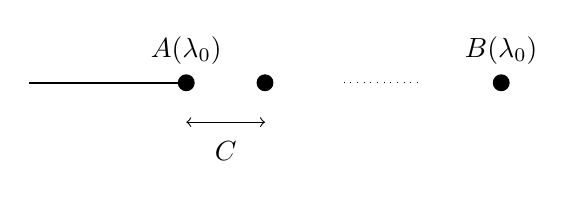
\begin{tikzpicture}
      \node[croot] at (2,0) [label=above:$A(\lambda_0)$] {};
      \node[croot] at (3,0) {};
      \node[croot] at (6,0) [label=above:$B(\lambda_0)$] {};
      \draw[thick] (0,0) to (2,0);
      \draw [dotted] (4,0) to (5,0);
      \draw[<->] (2,-0.5) -- (3,-0.5);
      \node at (2.5,-0.5) [label=below:$C$] {};
  \end{tikzpicture}
	
	$A(\lambda_0)$, $B(\lambda_0)$ and $C(\lambda_0)$ are real numbers expressible in terms of certain root systems $Q(\lambda_0)$ and $R(\lambda_0)$ associated to $\lambda_0$
	\item \emph{level of reduction}: $\lambda=(B - nC)\zeta + \lambda_0 \in \Lambda_r$ we have $l(\lambda) =n+1$
\end{itemize}
\end{frame}

\begin{frame}{Classification -- cone decomposition}
$a=(Q(\lambda_0), R(\lambda_0), l(\lambda_0))$ for ``reducible'' unitarizable highest weight module

$C_a$  -- integral cone of $\lie{k}$-dominant integral elements in $\lie{h}^*_\R$ which are orthogonal to elements in $R$

The set of reduction points $\Lambda_r$ is the disjoint union of translated integral cones $\lambda_a + C_a$.
\end{frame}


\begin{frame}{Enright's formula}

\begin{definition}\label{def:cohomology_roots}
Let $\Psi_\lambda$ be the set of roots orthogonal to $\lambda+\rho$.

\pause

 Denote by $\roots_{n,\lambda}^+$ the roots which satisfy the following conditions
 \begin{enumerate}
    \item $\alpha \in \roots_n^+$ and $(\lambda+\rho,\alpha^\vee)$ is a positive integer;
    \item $\alpha$ is orthogonal to $\Psi_\lambda$;
    \item $\alpha$ is short if there exist a long root in $\Psi_\lambda$.
 \end{enumerate}

\pause 

 Let $W_\lambda$ be the subgroup of $W$ which is generated by reflections $s_\alpha$ for $\alpha\in \roots_{n,\lambda}^+$.

\pause 

 Let $\roots_\lambda$ be the subset of $\roots$ of elements $\beta$ with $s_\beta\in W_\lambda$ and let $\roots_{\lambda,c} = \roots_c \cap \roots_\lambda$, $\roots_{\lambda,c}^+ = \roots_{\lambda,c} \cap \roots^+$.

\pause 

 Finally, define  $W^{c,i}_\lambda = \{ w \in W_\lambda \, |\, w \rho \text{ is } \roots^+_{\lambda, c}\text{-dominant and } l_\lambda(w)=i \}$.
\end{definition}

\end{frame}

\begin{frame}{Enright's formula -- continued}
\begin{theorem}[Theorem 3.7 of \cite{davidson_differential_1991}]
 For unitarizable highest weight modules $L(\lambda)$ and for $i\in \mathbb{N}$ we have
\begin{equation*}
 H^i(\lie{p}_+, L(\lambda))\simeq \bigoplus_{w\in W^{c,i}_\lambda} F(\overline{w(\lambda+\rho)} - \rho)
\end{equation*}
where  $\overline{\lambda}$ is the unique $\roots_c^+$-dominant element in the $W_c$ orbit of $\lambda$.
\end{theorem}

\end{frame}


\begin{frame}{Example -- scalar products with positive roots}
$\mathrm{SO}^*(16)$: $\lambda = \left(a_{5} + 1\right)\omega_{5} + a_6\omega_6 + a_7\omega_7 - \left(2 \, a_{5} + 2 \, a_{6} + a_{7} + 8\right)\omega_{8}$
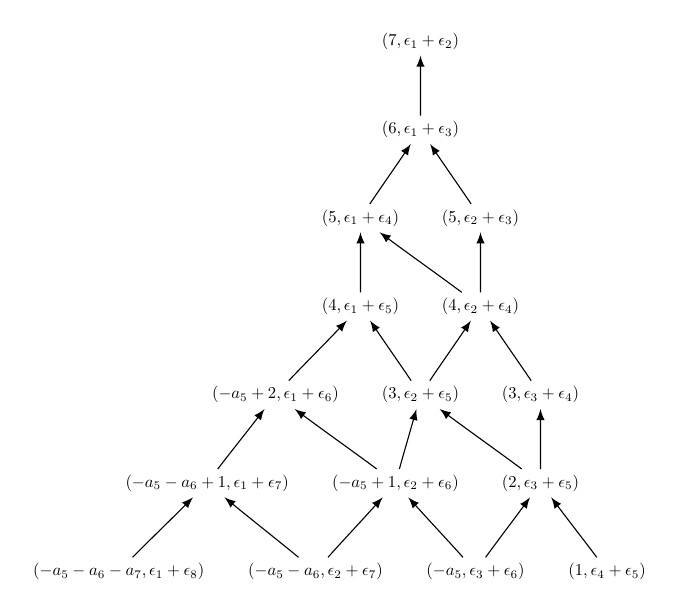
\begin{tikzpicture}[>=latex,line join=bevel,scale=0.6, every node/.style={transform shape}]
%%
\node (node_2) at (308.5bp,61.5bp) [draw,draw=none] {$(2, \epsilon_{3} + \epsilon_{5})$};
  \node (node_4) at (173.5bp,8.5bp) [draw,draw=none] {$(-a_{5} - a_{6}, \epsilon_{2} + \epsilon_{7})$};
  \node (node_3) at (269.5bp,8.5bp) [draw,draw=none] {$(-a_{5}, \epsilon_{3} + \epsilon_{6})$};
  \node (node_9) at (200.5bp,220.5bp) [draw,draw=none] {$(5, \epsilon_{1} + \epsilon_{4})$};
  \node (node_8) at (149.5bp,114.5bp) [draw,draw=none] {$(-a_{5} + 2, \epsilon_{1} + \epsilon_{6})$};
  \node (node_7) at (221.5bp,61.5bp) [draw,draw=none] {$(-a_{5} + 1, \epsilon_{2} + \epsilon_{6})$};
  \node (node_6) at (236.5bp,114.5bp) [draw,draw=none] {$(3, \epsilon_{2} + \epsilon_{5})$};
  \node (node_5) at (308.5bp,114.5bp) [draw,draw=none] {$(3, \epsilon_{3} + \epsilon_{4})$};
  \node (node_14) at (236.5bp,326.5bp) [draw,draw=none] {$(7, \epsilon_{1} + \epsilon_{2})$};
  \node (node_13) at (348.5bp,8.5bp) [draw,draw=none] {$(1, \epsilon_{4} + \epsilon_{5})$};
  \node (node_12) at (108.5bp,61.5bp) [draw,draw=none] {$(-a_{5} - a_{6} + 1, \epsilon_{1} + \epsilon_{7})$};
  \node (node_11) at (200.5bp,167.5bp) [draw,draw=none] {$(4, \epsilon_{1} + \epsilon_{5})$};
  \node (node_10) at (55.5bp,8.5bp) [draw,draw=none] {$(-a_{5} - a_{6} - a_{7}, \epsilon_{1} + \epsilon_{8})$};
  \node (node_1) at (272.5bp,167.5bp) [draw,draw=none] {$(4, \epsilon_{2} + \epsilon_{4})$};
  \node (node_0) at (272.5bp,220.5bp) [draw,draw=none] {$(5, \epsilon_{2} + \epsilon_{3})$};
  \node (node_15) at (236.5bp,273.5bp) [draw,draw=none] {$(6, \epsilon_{1} + \epsilon_{3})$};
  \draw [black,->] (node_12) ..controls (120.42bp,77.332bp) and (129.52bp,88.646bp)  .. (node_8);
  \draw [black,->] (node_8) ..controls (164.56bp,130.56bp) and (176.35bp,142.35bp)  .. (node_11);
  \draw [black,->] (node_10) ..controls (71.149bp,24.558bp) and (83.403bp,36.35bp)  .. (node_12);
  \draw [black,->] (node_6) ..controls (246.92bp,130.26bp) and (254.79bp,141.41bp)  .. (node_1);
  \draw [black,->] (node_1) ..controls (250.71bp,183.93bp) and (232.91bp,196.54bp)  .. (node_9);
  \draw [black,->] (node_3) ..controls (280.84bp,24.332bp) and (289.49bp,35.646bp)  .. (node_2);
  \draw [black,->] (node_4) ..controls (187.6bp,24.483bp) and (198.55bp,36.114bp)  .. (node_7);
  \draw [black,->] (node_9) ..controls (210.92bp,236.26bp) and (218.79bp,247.41bp)  .. (node_15);
  \draw [black,->] (node_0) ..controls (262.08bp,236.26bp) and (254.21bp,247.41bp)  .. (node_15);
  \draw [black,->] (node_11) ..controls (200.5bp,182.81bp) and (200.5bp,193.03bp)  .. (node_9);
  \draw [black,->] (node_7) ..controls (225.73bp,76.88bp) and (228.78bp,87.262bp)  .. (node_6);
  \draw [black,->] (node_13) ..controls (336.87bp,24.332bp) and (327.99bp,35.646bp)  .. (node_2);
  \draw [black,->] (node_15) ..controls (236.5bp,288.81bp) and (236.5bp,299.03bp)  .. (node_14);
  \draw [black,->] (node_5) ..controls (298.08bp,130.26bp) and (290.21bp,141.41bp)  .. (node_1);
  \draw [black,->] (node_1) ..controls (272.5bp,182.81bp) and (272.5bp,193.03bp)  .. (node_0);
  \draw [black,->] (node_7) ..controls (199.71bp,77.935bp) and (181.91bp,90.539bp)  .. (node_8);
  \draw [black,->] (node_2) ..controls (286.71bp,77.935bp) and (268.91bp,90.539bp)  .. (node_6);
  \draw [black,->] (node_6) ..controls (226.08bp,130.26bp) and (218.21bp,141.41bp)  .. (node_11);
  \draw [black,->] (node_3) ..controls (255.4bp,24.483bp) and (244.45bp,36.114bp)  .. (node_7);
  \draw [black,->] (node_2) ..controls (308.5bp,76.805bp) and (308.5bp,87.034bp)  .. (node_5);
  \draw [black,->] (node_4) ..controls (154.02bp,24.784bp) and (138.37bp,37.061bp)  .. (node_12);
%
\end{tikzpicture}
\end{frame}


\begin{frame}{Example -- nilpotent cohomology for $ \lie{so}(2,2n-2)$}

$\lie{g} = \lie{so}(2,2n-2)$ with $\lambda = (2-n)\omega_1$

$\lambda + \rho = (1,n-2,\ldots,1,0)$

 $\Psi_\lambda^+ = \{ \epsilon_1 - \epsilon_{n-1}\}$

The only noncompact root that is orthogonal to $\epsilon_1 -  \epsilon_{n-1}$ and whose scalar product with $\lambda + \rho$ is positive integral is $\alpha = \epsilon_1 + \epsilon_{n-1}$. 

Thus we get $\roots_{n,\lambda}^+ = \epsilon_1 + \epsilon_{n-1} = \roots_\lambda$. It follows that
\begin{align*}
 H^0(\lie{p}_-,L((2-n)\omega_1)) &= F((2-n)\omega_1)\\
 H^1(\lie{p}_-,L((2-n)\omega_1)) &= F(-n\omega_1)\\
 H^i(\lie{p}_-,L((2-n)\omega_1)) &= 0 \text{ for } i\geq 2.
\end{align*} 
\end{frame}

\begin{frame}{Example -- nilpotent cohomology for $ \lie{so}(2,2n-1)$}


Similarly for $\lie{g} = \lie{so}(2,2n-1)$ and $\lambda = (3/2 - n)\omega_1$ and we get that in that case
\begin{align*}
 H^0(\lie{p}_-,L((3/2-n)\omega_1)) &= F((3/2-n)\omega_1)\\
 H^1(\lie{p}_-,L((3/2-n)\omega_1)) &= F((-1/2-n)\omega_1)\\
 H^i(\lie{p}_-,L((3/2-n)\omega_1)) &= 0 \text{ for } i\geq 2.
\end{align*}

\end{frame}


\section{Conclusion}


\begin{frame}{Summary}

\begin{itemize}
 \item uniform and elementary construction of octonionic planes 
 \item generalization of Calderbank--Diemer construction to unitarizable highest weight modules
 \item software for nilpotent cohomology calculations 
 \item complete nilpotent cohomology of unitarizable highest weight modules in conformal case / partial results elsewhere
\end{itemize}

\end{frame}


{\setbeamercolor{palette primary}{fg=black, bg=white}

\begin{frame}[standout]

Thank you for your attention!

\end{frame}

}


\appendix


\begin{frame}[allowframebreaks]{References}


% \bibliography{../thesis}

% \bibliographystyle{abbrv}

\printbibliography


\end{frame}



\begin{frame}{F-method}


\end{frame}


\end{document}